%%%%%%%%%%%%%%%%%%%%%%%%%%%%%%%%%%%%%%%%%
%
% (c) 2018 by Jennifer Laaser
%
% This work is licensed under the Creative Commons Attribution-NonCommercial-ShareAlike 4.0 International License. To view a copy of this license, visit http://creativecommons.org/licenses/by-nc-sa/4.0/ or send a letter to Creative Commons, PO Box 1866, Mountain View, CA 94042, USA.
%
% The current source for these materials is accessible on Github: https://github.com/jlaaser/pogil-polymers
%
%%%%%%%%%%%%%%%%%%%%%%%%%%%%%%%%%%%%%%%%%

\documentclass[book]{pogil}

%%%%%%%%%%%%%%%%% DOCUMENT INFORMATION %%%%%%%%%%%%%%%%%%%%%%%%

\author{Jennifer Laaser}
\institution{University of Pittsburgh}
\title{POGIL Polymers}
\subtitle{Guided-Inquiry Activities \\for Polymer Chemistry and Polymer Physics}
\date{\today}

\copyrightshort{
\includegraphics[width=0.1\textwidth]{by-nc-sa} J. Laaser 2018}
\copyrightfulltext{
	\textcopyright 2018 by Jennifer Laaser. Except where otherwise noted, \thetitle\ is made available under a Creative Commons Attribution-NonCommercial-ShareAlike 4.0 International License: \url{http://creativecommons.org/licenses/by-nc-sa/4.0/}

	The current source for these materials is accessible on Github:\\ 		\url{https://github.com/jlaaser/pogil-polymers}
}
\copyrightgraphic{by-nc-sa}


%%%%%%%%%%%%%%%%%%%%%%%%%%%%%%%%%%%%%%%%%%%%%%%%%%%%%%%%%%%%%%
%%%%%%%%%%%%%%%%%%%%%%%%%%%%%%%%%%%%%%%%%%%%%%%%%%%%%%%%%%%%%%

\begin{document}

\frontmatter
\pagestyle{empty}
\titlepage
\clearpage

\copyrightpage
\clearpage

\tableofcontents*
\clearpage

%\chapter{Introduction}

%\lipsum[1-12]

\mainmatter
\pagestyle{fancy}

\part{Introduction to Polymers}

	\chapter{From Molecules to Polymers}

\part{Polymer Chemistry}

	\chapter{Fundamentals of Polymer Chemistry}

	\chapter{Step-Growth Polymerizations}
		%%%%%%%%%%%%%%%%%%%%%%%%%%%%%%%%%%%%%%%%%
%
% (c) 2019 by Jennifer Laaser
%
% This work is licensed under the Creative Commons Attribution-NonCommercial-ShareAlike 4.0 International License. To view a copy of this license, visit http://creativecommons.org/licenses/by-nc-sa/4.0/ or send a letter to Creative Commons, PO Box 1866, Mountain View, CA 94042, USA.
%
% The current source for these materials is accessible on Github: https://github.com/jlaaser/pogil-polymers
%
%%%%%%%%%%%%%%%%%%%%%%%%%%%%%%%%%%%%%%%%%

\renewcommand{\figpath}{content/polymchem/stepgrowth/stepgrowth-chemistries/figs}
\renewcommand{\labelbase}{stepgrowth-chem}

\begin{activity}{Chemistries of Step-Growth Polymerizations}

\begin{instructornotes}

	This activity introduces students to key chemistries used for step-growth polymerizations.
	
	After completing this activity, students will be able to:
			\begin{enumerate}
				\item Identify major classes of polymers produced by step-growth polymerization
				\item Determine the polymer produced by a given monomer or monomer pair, and determine the monomer(s) necessary to produce a target polymer
				\item Determine whether or not a reaction qualifies as a condensation polymerization, and if so, identify the small molecule released
			\end{enumerate}
	
			
	\subsection*{Activity summary:}
	\begin{itemize}
		\item \textbf{Activity type:} Learning Cycle
		\item \textbf{Content goals:} Chemistries of step-growth polymerizations
		\item \textbf{Process goals:} %https://pogil.org/uploads/attachments/cj54b5yts006cklx4hh758htf-process-skills-official-pogil-list-2015-original.pdf
			written communication, critical thinking, information processing
		\item \textbf{Duration:} approx. 45 minutes
		\item \textbf{Instructor preparation required:} none beyond knowledge of relevant content
		\item \textbf{Related textbook chapters:}
			\begin{itemize}
				\item \emph{Polymer Chemistry} (Hiemenz \& Lodge): Table 1.2 and sections 2.2.1, 2.5, and 2.6
			\end{itemize}
	\end{itemize}

\end{instructornotes}

	%\textbf{Focus question:} Put a central question for the students to consider through this exercise here.

\begin{model}[Synthesis of a Polyester]
\label{\labelbase:mdl:polyester}

	Esterification reactions are a common type of reaction used to produce polymers by step-growth polymerization.
	In a typical esterification reaction, an alcohol and a carboxylic acid react to form an ester bond:
	
	\centerline{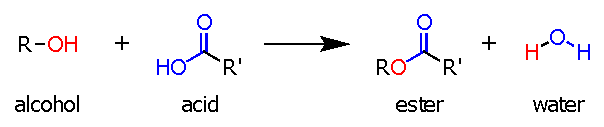
\includegraphics[width=0.7\textwidth]{\figpath/model1_ester-general.pdf}}
	
	One example of a polymerization reaction using this chemistry is the synthesis of poly(6-hydroxycaproic acid) from 6-hydroxycaproic acid monomers:
	
	\centerline{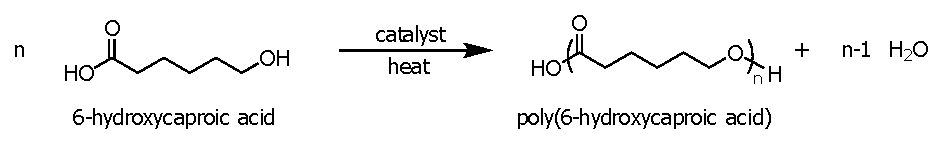
\includegraphics[width=0.9\textwidth]{\figpath/model1_P6HCA.pdf}}

\end{model}


\begin{ctqs}

	\question Consider the 6-hydroxycaproic acid monomer shown in Model \ref{\labelbase:mdl:polyester}: \label{\labelbase:ctq:label-6hcpa}
	
		\begin{enumerate}
			\item As drawn, what type of functional group is on the \emph{left} side of the monomer?
			
				\begin{solution}[1in]
					carboxylic acid (``acid'' is also fine)
				\end{solution}
			
			\item As drawn, what type of functional group is on the \emph{right} side of the monomer?
			
				\begin{solution}[1in]
					alcohol (or hydroxyl)
				\end{solution}
		\end{enumerate}
		
\end{ctqs}

\begin{infobox}

	When a monomer used in a step-growth polymerization has different reactive functional groups on each end, it is called an ``AB-type'' monomer.
	
	When a monomer used in a step-growth polymerization has the same reactive functional group on each end, it is called an ``AA-type'' or ``BB-type'' monomer.

\end{infobox}

\begin{ctqs}
		
		\question Would you classify the poly(6-hydroxycaproic acid) monomer used in this synthesis as an AA-type monomer or an AB-type monomer?  Briefly explain your answer in 1-2 complete sentences.
			
				\begin{solution}[1.75in]
					This is an AB-type monomer, because it has two different reactive functional groups in the same monomer.
				\end{solution}
		
		\question The synthesis of a short 6-hydroxycaproic acid oligomer from three monomers is shown explicitly, below: \label{\labelbase:ctq:6hcpa-oligomer}
	
\vspace{0.25in}	\centerline{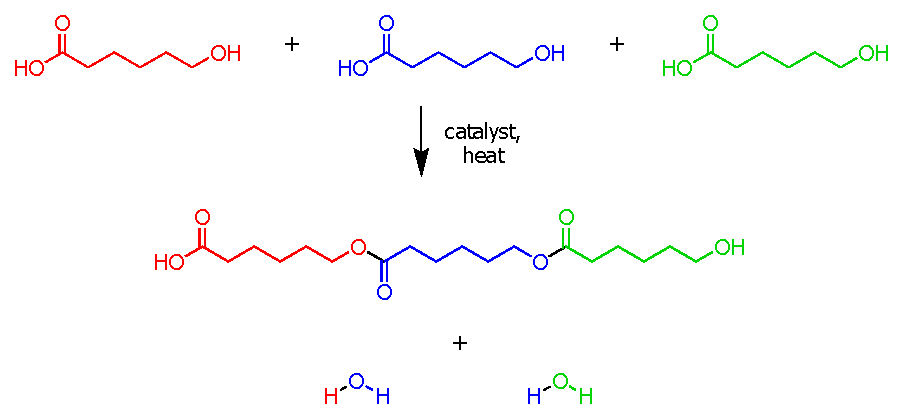
\includegraphics[width=0.9\textwidth]{\figpath/model1_3oligomer-explicit.pdf}}
The molecules are shaded and color-coded so that you can see which atoms in the oligomer came from which monomer.
		
		\begin{enumerate}
		
			\item What type of bonds connect the different monomers in the polymer backbone?
			
				\begin{solution}[1.5in]
					The monomers are connected by ester bonds.
				\end{solution}
		
			\item Explain, in one or two complete sentences, why you think we classify this polymer as a ``polyester'':
			
				\begin{solution}[2in]\instructordisplay{
					We call this polymer a ``polyester'' because it has ester groups in the polymer backbone.
					
					Note: the fact that they are in the backbone is important; if the ester groups are only in the sidechains, the polymer is \emph{not} a polyester - students will address this point in CTQ \ref{\labelbase:ctq:PMA}.
				}\end{solution}
	
			\item When we write the structure of this oligomer as
	
	\centerline{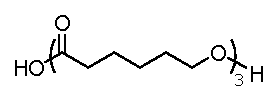
\includegraphics[width=0.25\textwidth]{\figpath/model1_3oligomer-shorthand.pdf}}
	\vspace{-3pt}
	how many different monomer molecules contribute to each repeat unit in the polymer chain?
			
				\begin{solution}[1in]
					one
				\end{solution}
		
			\item Explain, in one or two complete sentences, why we generally abbreviate the product of this reaction as
	
	\centerline{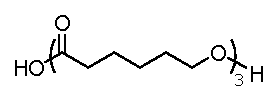
\includegraphics[width=0.25\textwidth]{\figpath/model1_3oligomer-shorthand.pdf}}
	
	rather than as
	
	\centerline{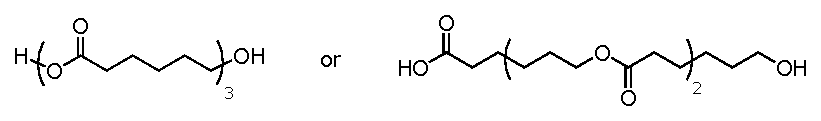
\includegraphics[width=0.7\textwidth]{\figpath/model1_incorrect-shorthand.pdf}}
			
				\begin{solution}[2in]
					We use the first notation because all of the atoms in a single repeat unit come from the same monomer (if you draw these parentheses on the color-coded molecules at the beginning of the question, each pair of parentheses will only have one color of atoms in it).  This is not true for the second and third options.
				\end{solution}
			
		\end{enumerate}
	
	\question Consider the following polymer:\label{\labelbase:ctq:PMA}
	
	\centerline{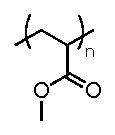
\includegraphics[width=0.1\textwidth]{\figpath/model1_PMA.pdf}}
	
		\begin{enumerate}
				
			\item Does this polymer have ester bonds in the polymer backbone?
			
				\begin{solution}[0.75in]
					No (they are only in the sidechains).
				\end{solution}
		
			\item Would you be able to produce this polymer by esterification reactions of small molecules?  Why or why not?
			
				\begin{solution}[2in]
					No.  This polymer (poly(methyl acrylate)) contains ester bonds, but they are only in the sidechains, not the backbone.  But when we produce a polymer from esterification reactions of small molecules, the ester bonds end up in the polymer backbone.
					
					Put another way, the backbone in this polymer only contains carbon-carbon bonds, which cannot be formed by esterification reactions.
				\end{solution}
			
			\item Based on your answers to the previous two questions, would you classify this polymer as a polyester?  Why or why not?
			
				\begin{solution}[2in]
					No, this is not a polyester because it does not contain ester bonds in the polymer backbone, and cannot be produced by esterification of small molecules.
				\end{solution}
			
		\end{enumerate}
		
\end{ctqs}
	

\clearpage
\begin{model}[Synthesis of a Polyamide]

Amidation reactions are another type of reaction used to produce polymers by step-growth polymerizations.
For example, acid chlorides can be reacted with primary amines to form an amide bond:
	
	\centerline{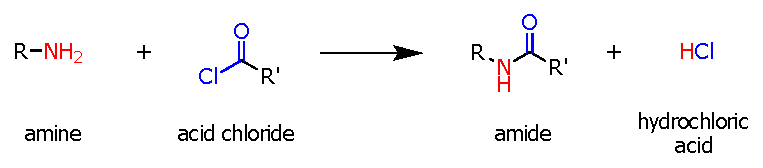
\includegraphics[width=0.7\textwidth]{\figpath/model2_amide-general.pdf}}

Commercially, this reaction is used to produce Nomex, a heat-resistant polymer used in oven mitts and firefighters' protective clothing, among other applications.
A reaction scheme for the synthesis of Nomex is shown below:
	
	\centerline{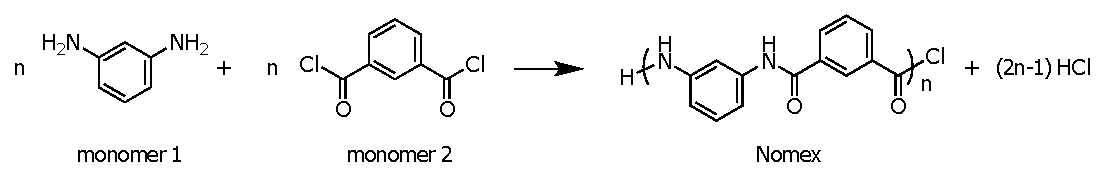
\includegraphics[width=0.9\textwidth]{\figpath/model2_Nomex.pdf}}

\end{model}

\begin{ctqs}
		\question Why is this polymer classified as a polyamide?
			
				\begin{solution}[1.5in]
					This polymer is classified as a polyamide because it has amide bonds in the polymer backbone.
				\end{solution}
		
		\question What functional groups does monomer 1 have?   Would you classify this monomer as an AA-type monomer or an AB-type monomer?
			
				\begin{solution}[0.75in]
					Monomer 1 has two amine groups.  Because it has two of the same reactive group, it is an AA-type monomer.
				\end{solution}
		
		\question What functional groups does monomer 2 have?   Would you classify this monomer as an AA-type monomer or an AB-type monomer?
			
				\begin{solution}[0.75in]
					Monomer 2 has two acid chloride groups.  Because it has two of the same reactive group, it is an AA-type monomer.
				\end{solution}
		
		\question Explain, in one or two complete sentences, why we might describe this reaction as an ``AA+BB''-type polymerization:
			
				\begin{solution}[1.75in]
					This polymer is formed from two AA-type monomers.  Since the two monomers are chemically different, we distinguish them by calling one the ``AA-type'' monomer and the other a ``BB-type'' monomer; thus, we call the polymerization an ``AA+BB''-type polymerization.
					
					This reaction is notably different from the AB-type polymerization in Model 1 because it requires two chemically distinct monomers; in the AB-type polymerization in Model 1, we only needed one type of monomer.
				\end{solution}
		
		\question How many monomers make up each repeat unit?
			
				\begin{solution}[1in]
					two
				\end{solution}
		
		\question A very similar reaction can be used to make Kevlar, the high-strength polymer used in bulletproof vests and cut-resistant gloves.  Given that Kevlar is produced from the following two monomers,
		
	
	\centerline{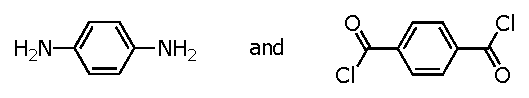
\includegraphics[width=0.5\textwidth]{\figpath/model2_Kevlar-monomers.pdf}}
		
		predict the structure of the Kevlar polymer:
			
				\begin{solution}[2.5in]
					\instructordisplay{\centerline{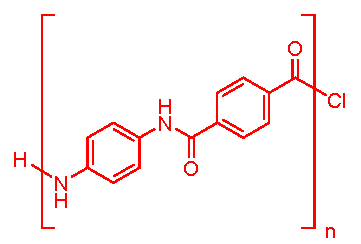
\includegraphics[width=0.4\textwidth]{\figpath/model2_Kevlar.pdf}}
					
					Note: for the purposes of this question, the repeat unit structure is more important than the end groups.  One potential set of end-groups is shown here, although practically speaking, the acid-chloride end group is unlikely to persist - it is very reactive, and would likely hydrolyze to a carboxylic acid.}
				\end{solution}
		
		\clearpage
		\question A similar chemistry can also be used to prepare nylon-6,6, a polymer used in many consumer goods.
		The structure of nylon-6,6 is shown below:
		
			\centerline{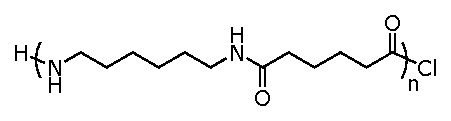
\includegraphics[width=0.45\textwidth]{\figpath/model2_nylon66.pdf}}
			
		What two monomers would you need to combine to make this polymer?
			
				\begin{solution}[2in]
					\instructordisplay{\centerline{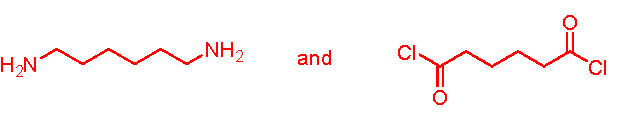
\includegraphics[width=0.6\textwidth]{\figpath/model2_nylon66-monomers.pdf}}}
				\end{solution}
			
\end{ctqs}
	
\begin{infobox}

A polymerization reaction is called a \emph{condensation} polymerization if the reaction produces a small-molecule byproduct that is not part of the polymer chain.

\end{infobox}
	
\begin{ctqs}
		\question Is the esterification reaction in Model 1 a condensation polymerization?  If so, what is the small-molecule byproduct that is produced?
			
				\begin{solution}[1in]
					Yes, the reaction in Model 1 is a condensation polymerization. It produces \ce{H2O}.
				\end{solution}
		
		\question Is the amidation reaction in Model 2 a condensation polymerization?  If so, what is the small-molecule byproduct that is produced?
			
				\begin{solution}[1in]
					Yes, the reaction in Model 2 is a condensation polymerization. It produces \ce{HCl}.
				\end{solution}
		
\end{ctqs}

\begin{model}[Other Chemistries used for Step-Growth Polymerization]
\label{\labelbase:model:otherstepgrowthchems}

Shown below are synthetic schemes for a variety of other commercially-important polymers produced by step-growth polymerization:

\vspace{0.1in}

\textbf{a) polycarbonate} (high transparency and impact resistance; used in DVDs, glasses, etc.)
		
			\centerline{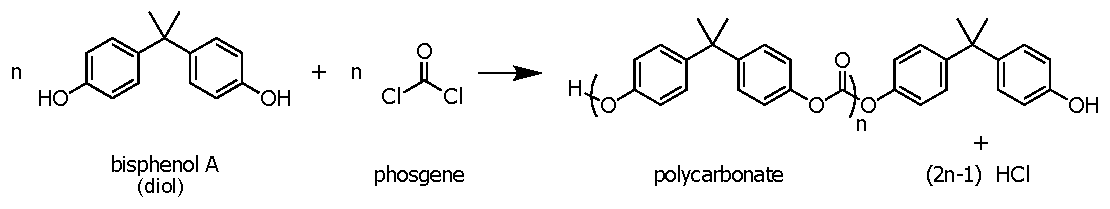
\includegraphics[width=\textwidth]{\figpath/model3_polycarbonate.pdf}}

\vspace{0.1in}

\textbf{b) polyurethanes} (foams; thermoplastic elastomers, e.g. spandex)
		
			\centerline{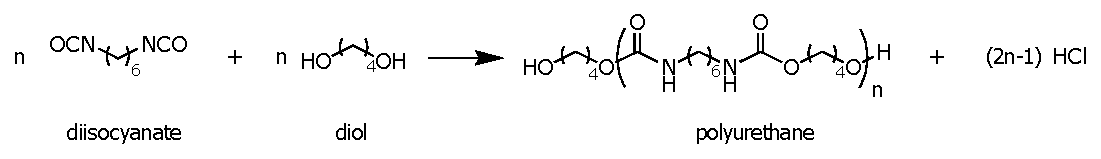
\includegraphics[width=0.9\textwidth]{\figpath/model3_polyurethane.pdf}}

\vspace{0.1in}

\textbf{c) epoxies} (adhesives; coatings)
		
			\centerline{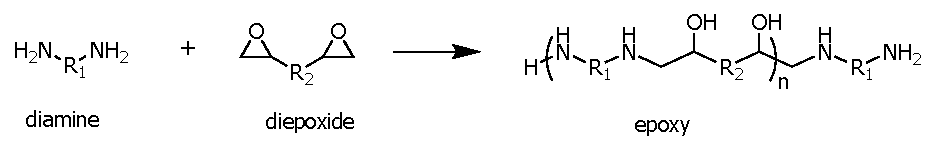
\includegraphics[width=\textwidth]{\figpath/model3_epoxy.pdf}}

\end{model}

\vspace{0.25in}
\begin{ctqs}

		\question Classify each of the reactions in the above Model as either an ``AB-type'' or ``AA+BB-type'' polymerization:
		
			\begin{enumerate}
				\item ~ \begin{solution}[0.6in]AA+BB-type\end{solution}
				\item ~ \begin{solution}[0.6in]AA+BB-type\end{solution}
				\item ~ \begin{solution}[0.6in]AA+BB-type\end{solution}
			\end{enumerate}
			
		% may need another question in here
		
		\clearpage
		\question Complete the following table for the polymerizations depicted in Models 1-3:
		
			\begin{center}
				\begin{tabular}{|c|c|c|c|c|}
				\hline
					Polymer & ``A'' reactive group & ``B'' reactive group & ``ab'' bond formed & \begin{tabular}{c}Small\\ Molecule\\Byproduct\end{tabular} \\\hline
					Polyester &						
						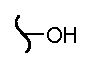
\includegraphics[width=0.12\textwidth]{\figpath/model3_hydroxyl.pdf} &
						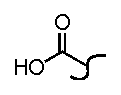
\includegraphics[width=0.15\textwidth]{\figpath/model3_acid.pdf} &
						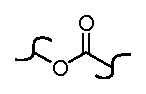
\includegraphics[width=0.15\textwidth]{\figpath/model3_ester.pdf}&
						\answer{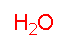
\includegraphics[width=0.08\textwidth]{\figpath/model3_H2O-red.pdf}}\\\hline
					Polyamide &
						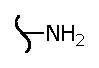
\includegraphics[width=0.12\textwidth]{\figpath/model3_amine.pdf} &
						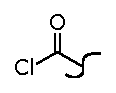
\includegraphics[width=0.15\textwidth]{\figpath/model3_acidchloride.pdf} &
						\answer{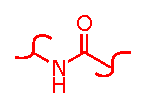
\includegraphics[width=0.15\textwidth]{\figpath/model3_amide-red.pdf}}&
						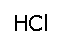
\includegraphics[width=0.08\textwidth]{\figpath/model3_HCl.pdf} \\\hline
					Polycarbonate &
						
\includegraphics[width=0.004\textwidth]{\figpath/model3_blank.pdf}\answer{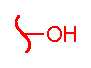
\includegraphics[width=0.12\textwidth]{\figpath/model3_hydroxyl-red-right.pdf}}&
						\answer{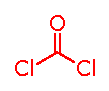
\includegraphics[width=0.15\textwidth]{\figpath/model3_phosgene-red.pdf}}&
						\answer{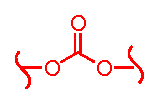
\includegraphics[width=0.15\textwidth]{\figpath/model3_carbonate-red.pdf}}& 
						\answer{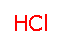
\includegraphics[width=0.08\textwidth]{\figpath/model3_HCl-red.pdf}}\\\hline
					Polyurethane &
						
\includegraphics[width=0.004\textwidth]{\figpath/model3_blank.pdf}\answer{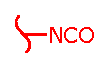
\includegraphics[width=0.12\textwidth]{\figpath/model3_isocyanate-red.pdf}}&
						\answer{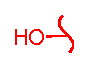
\includegraphics[width=0.12\textwidth]{\figpath/model3_hydroxyl-red-left.pdf}}& 
						\answer{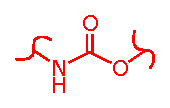
\includegraphics[width=0.15\textwidth]{\figpath/model3_urethane-red.pdf}}&
						\answer{none}\\\hline
					Epoxy &
						
\includegraphics[width=0.004\textwidth]{\figpath/model3_blank.pdf}\answer{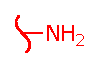
\includegraphics[width=0.12\textwidth]{\figpath/model3_amine-red.pdf}}&
						\answer{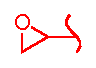
\includegraphics[width=0.12\textwidth]{\figpath/model3_epoxide-red.pdf}}&
						\answer{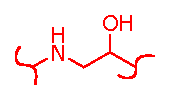
\includegraphics[width=0.15\textwidth]{\figpath/model3_epoxy-red.pdf}}&
						\answer{none} \\\hline
				\end{tabular}
			\end{center}
			
		\vspace{0.25in}
		\question Which of the above polymerization reactions would you classify as condensation polymerizations?  Briefly explain your answer in 1-2 complete sentences.
			
				\begin{solution}[2in]
					The first three reactions (formation of polyesters, polyamides, and polycarbonates) form small-molecule byproducts, so are condensation polymerizations.
					
					The last two reactions (formation of polyurethanes and epoxies) do not form small-molecule byproducts, so are not condensation polymerizations.
				\end{solution}
			
\end{ctqs}
	

\clearpage
\begin{exercises}

		%\exercise (alternate esterification and amidation chemistries? see H&L Tables 2.3 and 2.4)
		
		\exercise \label{\labelbase:exc:AABBester} Although the polymers formed by AB-type and AA+BB-type step-growth polymerizations are similar, there are some subtle but important differences.
			Consider the synthesis of a polyester from the following two monomers:
			
			\centerline{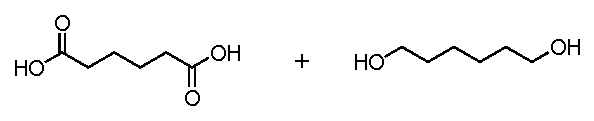
\includegraphics[width=0.6\textwidth]{\figpath/exercises_polyester-AABB-monomers.pdf}}	
			
			\begin{enumerate}
				\item Draw the structure of the polymer that would be formed from this pair of monomers.
					
					\begin{solution}\instructordisplay{
						\centerline{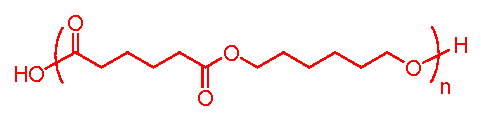
\includegraphics[width=0.4\textwidth]{\figpath/exercises_polyester-AABB-shorthand.pdf}}
					}\end{solution}
					
				\item Compare this structure to the polymer produced from the AB-type monomer in Model 1 (hint: you may find it useful to explicitly draw out a few repeat units).  Are they the same, or different?  If they are different, briefly describe what is different about the two structures.
					
					\begin{solution}\instructordisplay{
						If we explicitly draw out two repeat units of the polymer produced from the AA+BB type monomers, we get something like this:
						
						\centerline{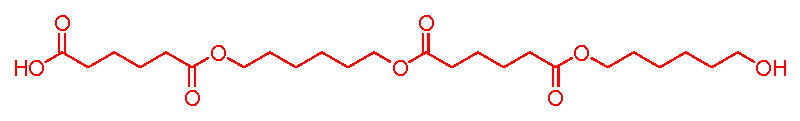
\includegraphics[width=0.7\textwidth]{\figpath/exercises_polyester-AABB-4oligo.pdf}}
						
						On the other hand, if we explicitly draw out the polymer produced from the AB-type monomers, we get
						
						\centerline{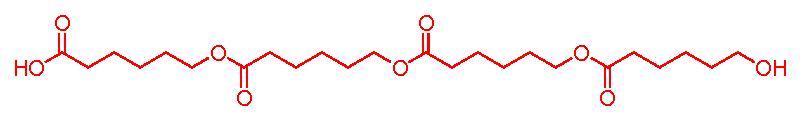
\includegraphics[width=0.7\textwidth]{\figpath/exercises_polyester-AB-4oligo.pdf}}
						
						These structures are very similar; however, as you will notice, the orientation of the ester groups is slightly different: in the polymer produced from AB-type monomers, every ester group is oriented in the same direction, while in the polymer produced from the AA+BB-type monomers, they alternate.
						
						Another consequence is that the effective spacing between carbonyl groups is constant in the polymer produced from AB-type monomers (there are 6 atoms separating each \ce{C=0}), while it varies in the polymer produced from AA+BB-type monomers (where the spacing alternates between 6 and 8 atoms separating each \ce{C=O} group).
						These differences will affect the physical properties of the polymers by changing - among other things - how easy it is for the chains to pack or align with each other.
						
					}\end{solution}
					
			\end{enumerate}
		
		\exercise One of the reasons that polyamides have such useful properties is that the amide groups can form hydrogen bonds between chains, as shown below:
			
			\centerline{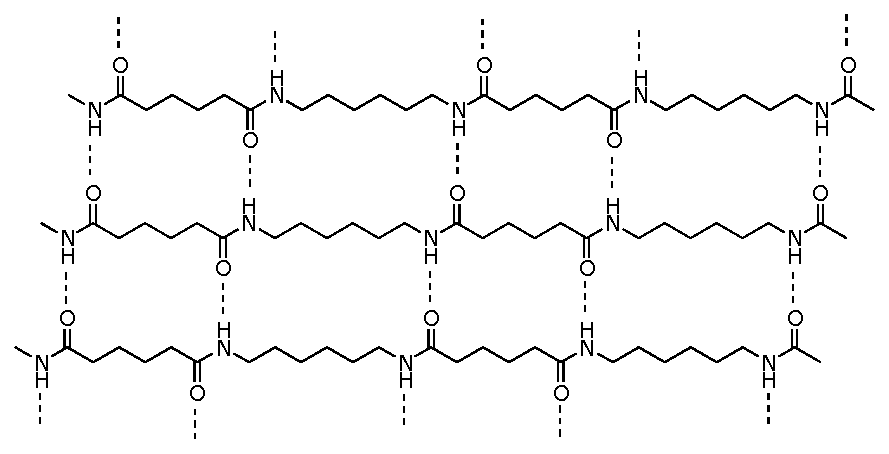
\includegraphics[width=0.7\textwidth]{\figpath/exercises_nylon-network-Hbond.pdf}}	
		
			These inter-chain hydrogen bonds significantly improve the mechanical properties (e.g. stiffness, resilience, etc.) of the material.
			
			Draw an analogous structure for the AA+BB-type polyester that you drew in Exercise \ref{\labelbase:exc:AABBester}.  Can this polymer form inter-chain hydrogen bonds?  Briefly explain your answer, and discuss how you expect the physical properties of the polyester to compare to those of the polyamide.
			
			\begin{solution}\instructordisplay{	
				The analogous structure for the AA+BB-type polyester is
			
			\centerline{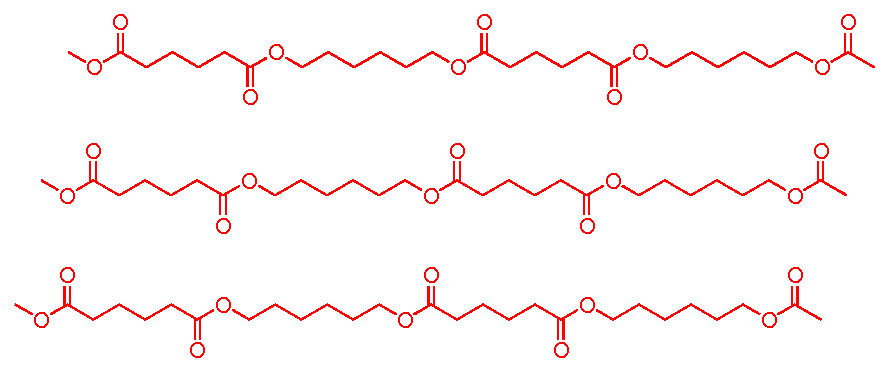
\includegraphics[width=0.8\textwidth]{\figpath/exercises_polyester-network.pdf}}	
			
				While the polyamide was able to form hydrogen bonds because amide \ce{NH} bond (which is polar, and has a partial positive charge on the hydrogen atom which can interact with the partial negative charge on the adjacent chain's carbonyl groups), the polyester lacks this feature - there is no \ce{OH} or \ce{NH} functionality, and it cannot form hydrogen bonds.
				
				Because the polyester does not form inter-chain hydrogen bonds, we should expect it to be much less mechanically stable - it will probably be softer and less robust.
				}\end{solution}
		
		%\exercise (phosgene alternatives for polycarbonate synthesis?)
		
		\exercise The epoxidation reaction shown in Model \ref{\labelbase:model:otherstepgrowthchems} formed a linear polymer with secondary amines.  However, secondary amines can also attack epoxides.  Draw out the polymer structure that you would expect to generate if this occurs.  How would you describe this polymer architecture?
		
			\begin{solution}\instructordisplay{
				If the secondary amines can also attack epoxides, they will generate branched polymers, as shown below:
			
			\centerline{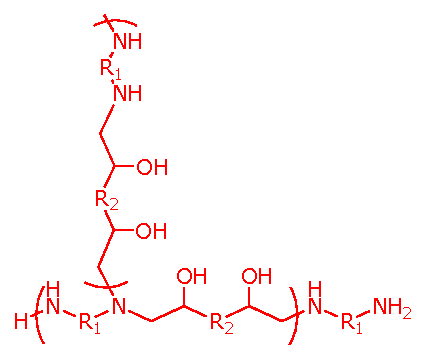
\includegraphics[width=0.4\textwidth]{\figpath/exercises_epoxy-branched.pdf}}	
				
				Note that the polymer chain can keep growing from this branch point, hence the parentheses on the branch as well as the main chain.			
				Eventually, this branch may react with another growing polymer chain, so if this process continues, we will eventually end up with a crosslinked polymer network.
				
				Note that most commercially available epoxy resins use amines with more than two nitrogens, so the monomer is not just a ``BB-type'' monomer, but may be a \ce{B3} or \ce{B4}-type monomer (where the subscript indicates the number of reactive B functional groups, or in this case, the number of amines).
				Similarly, while students were only asked to consider linear polyurethanes in this activity, commercial polyurethane foams typically contain ``polyols'' with 3 or more hydroxyl groups to promote crosslinking.
				
				The formation of networks from multi-functional monomers will be considered in more detail in a later activity.
				
			}\end{solution}
		
\end{exercises}
	
\end{activity}
		%%%%%%%%%%%%%%%%%%%%%%%%%%%%%%%%%%%%%%%%%
%
% (c) 2018 by Jennifer Laaser
%
% This work is licensed under the Creative Commons Attribution-NonCommercial-ShareAlike 4.0 International License. To view a copy of this license, visit http://creativecommons.org/licenses/by-nc-sa/4.0/ or send a letter to Creative Commons, PO Box 1866, Mountain View, CA 94042, USA.
%
% The current source for these materials is accessible on Github: https://github.com/jlaaser/pogil-polymers
%
%%%%%%%%%%%%%%%%%%%%%%%%%%%%%%%%%%%%%%%%%

\renewcommand{\figpath}{content/polymchem/stepgrowth/Mn-and-stoich/figs}

\begin{activity}[Degree of Polymerization in Step-Growth Polymerizations]

\begin{instructornotes}

	This activity introduces students to key concepts related to the degree of polymerization and stoichiometric balance in step-growth polymerizations.
	
	After completing this activity, students will be able to:
			\begin{enumerate}
				\item Calculate the number-average degree of polymerization for stoichiometrically-balanced step-growth polymerizations of `AB' or `AA+BB' monomer mixtures
				\item Explain what it means for a reaction to be stoichiometrically-balanced
				\item Describe the consequences of stoichiometric imbalance in terms of (a) the degree of polymerization and (b) the end-group functionality of the polymer chains.
			\end{enumerate}
	This activity will prepare students for follow-up activities on the chemistry, equilibria, kinetics, and molecular-weight distributions of step-growth polymerizations.
			
	\subsection*{Activity summary:}
	\begin{itemize}
		\item \textbf{Activity type:} Learning Cycle
		\item \textbf{Content goals:} Stoichiometry and degree of polymerization in step-growth polymerizations
		\item \textbf{Process goals:} %https://pogil.org/uploads/attachments/cj54b5yts006cklx4hh758htf-process-skills-official-pogil-list-2015-original.pdf
			written communication, critical thinking, information processing
		\item \textbf{Duration:} approx. 45-50 minutes without class discussion
		\item \textbf{Instructor preparation required:} none beyond knowledge of relevant content
		\item \textbf{Related textbook chapters:}
			\begin{itemize}
				\item \emph{Polymer Chemistry} (Hiemenz \& Lodge): sections 2.2 and 2.7
			\end{itemize}
	\end{itemize}

\end{instructornotes}

	%\textbf{Focus question:} Put a central question for the students to consider through this exercise here.

\begin{model}[Polymerization of ``AB''-Type Monomers]

The simplest type of step-growth polymerization is one in which each monomer has one ``A''-type reactive group and one ``B''-type reactive group.
These types of monomers are referred to as ``AB''-type monomers.

In each step of the polymerization, an ``A'' group on one molecule reacts with a ``B'' group on another molecule to form an ``ab'' bond, as shown below:

\vspace{0.1in}
\centerline{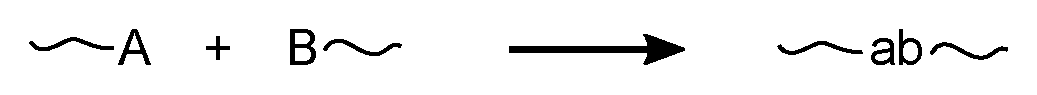
\includegraphics[width=0.6\textwidth]{\figpath/ABrxn.pdf}}

For example, for a simple reaction mixture containing 8 ``AB''-type monomers, the evolution of the reaction mixture might look something like this:

\vspace{0.1in}
\centerline{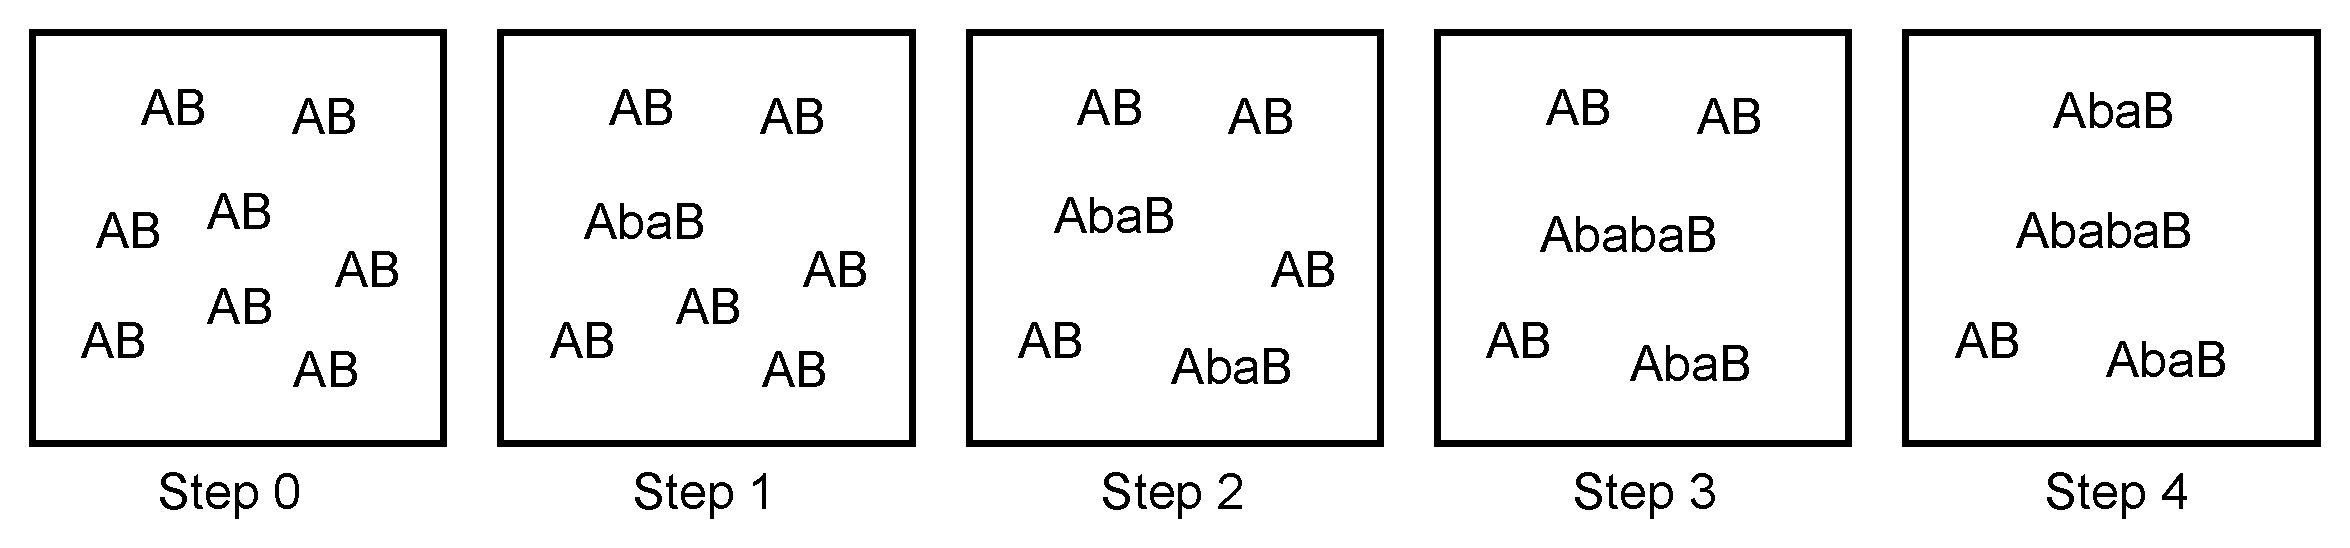
\includegraphics[width=0.9\textwidth]{\figpath/ABpolym.pdf}}

\end{model}

\begin{ctqs}

	\question \label{ctq:ABtable} For the reaction mixture shown in Model 1, fill out the following table:
	
			\begin{center}
				\renewcommand{\arraystretch}{3}
				\begin{tabular}{|c|c|c|}
					\hline
					\textbf{Step} &  \textbf{Number of unreacted ``A'' groups} & \textbf{Number of molecules} \\\hline
					0 & \answer{8} & \answer{8} \\\hline
					1 & \answer{7} & \answer{7}  \\\hline
					2 & \answer{6} & \answer{6}  \\\hline
					3 & \answer{5} & \answer{5}  \\\hline
					4 & \answer{4} & \answer{4}  \\\hline
				\end{tabular}
			\end{center}
		
	\question Explain, in a complete sentence, how the number of molecules in the mixture is related to the number of unreacted ``A'' groups.
		
		\begin{solution}[1in]
			The number of molecules in the mixture is exactly equal to the number of unreacted `A' groups at each step of the reaction.
		\end{solution}
		
		\question The number-average degree of polymerization, $N_n$, is the total number of \emph{monomers} divided by the total number of \emph{molecules}.  Remembering that we started with 8 monomers, calculate the number-average degree of polymerization for each step shown in Model 1.
		
			\begin{center}
				\renewcommand{\arraystretch}{4}
				\begin{tabular}{|c|c|c|c|c|c|}
					\hline
					\textbf{~~Step~~} &  \textbf{~~~~~0~~~~~} & \textbf{~~~~~1~~~~~} & \textbf{~~~~~2~~~~~} & \textbf{~~~~~3~~~~~} & \textbf{~~~~~4~~~~~} \\\hline
					$\mathbf{N_n}$ & \answer{8} & \answer{8/7=1.14} & \answer{8/6=1.33} & \answer{8/5=1.6} & \answer{8/4=2} \\\hline
				\end{tabular}
			\end{center}
		
		\question Suppose that you had initially started with 100 monomers.  Then, suppose that at some time later, you had only 8 unreacted ``A'' groups left.
		
			\begin{enumerate}
				\item How many molecules would there be in the reaction mixture at this point?
				
					\begin{solution}[0.5in]
						8
					\end{solution}
				
				\item What would the number-average degree of polymerization be at this point?
				
					\begin{solution}[0.5in]
						100/8 = 12.5
					\end{solution}
			\end{enumerate}
			
		\question More generally, suppose you started with $v_A^0$ monomers, and at some time later, you had only $v_A$ unreacted ``A'' groups left.  What would the number average-degree of polymerization be at this point, in terms of $v_A^0$ and $v_A$?
				
					\begin{solution}[0.5in]
						$N_n = \frac{v_A^0}{v_A}$
					\end{solution}
		
		\vspace{1in}
		
\end{ctqs}
	
\begin{infobox}

Usually, we find it more useful to work in terms of the \emph{fraction} of all ``A'' groups that have reacted, rather than the total \emph{number} of ``A'' groups that have reacted.  In step-growth polymerizations, we refer to the fraction of ``A'' groups that have reacted as the ``extent of reaction'', $p$.

\end{infobox}
	
\begin{ctqs}
		\question If we start with $v_A^0$ ``A'' groups, how many of the ``A'' groups will have \emph{reacted} when the extent of reaction is equal to $p$?
		
		\begin{solution}[1in]
			$p v_A^0$
		\end{solution}
		
		\question How many ``A'' groups are still \emph{unreacted} when the extent of reaction is equal to $p$?
		
		\begin{solution}[1in]
			$v_A = v_A^0 - p v_A^0 = (1-p)v_A^0$
		\end{solution}
		
		\question Using your answers to critical thinking questions 5, 6, and 7, derive an expression for $N_n$ in terms of $p$.
		
		\begin{solution}[1in]
			$N_n = \frac{v_A^0}{v_A} = \frac{v_A^0}{(1-p)v_A^0} = \frac{1}{1-p}$
		\end{solution}
		
\end{ctqs}

\begin{model}[Polymerization of ``AA'' and ``BB''-Type Monomers]

Now, let's consider a slightly more complicated reaction, with two different types of monomers that each have \emph{either} two ``A'' reactive groups \emph{or} two ``B'' type reactive groups.
We call monomers with two ``A'' groups ``AA''-type monomers, and we call monomers with two ``B'' groups ``BB''-type monomers.

Suppose we start with 4 ``AA''-type monomers and 4 ``BB''-type monomers.
In this case, the evolution of the reaction mixture might look something like this:

\vspace{0.1in}
\centerline{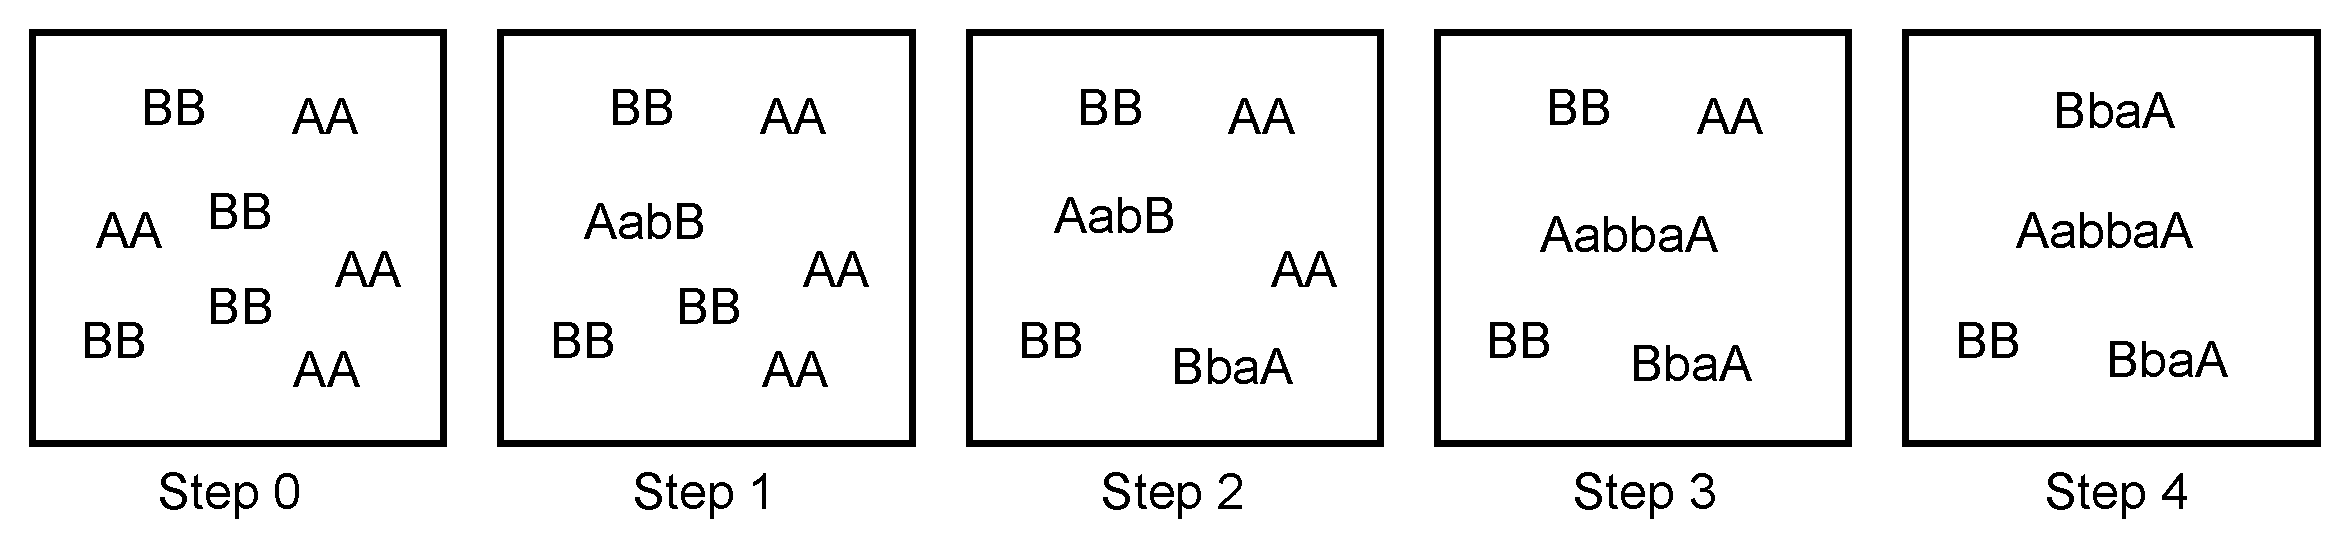
\includegraphics[width=0.9\textwidth]{\figpath/AABBpolym.pdf}}

\end{model}

\begin{ctqs}
		\question \label{ctq:AABBtable} For the reaction mixture shown in Model 2, fill out the following table:
		
			\begin{center}
				\renewcommand{\arraystretch}{3}
				\begin{tabular}{|c|c|c|c|}
					\hline
					\textbf{Step} &  \textbf{Number of unreacted ``A'' groups} & \textbf{Number of molecules} & ~~~~$\mathbf{N_n}$~~~~\\\hline
					0 & \answer{8} & \answer{8} & \answer{8/8=1} \\\hline
					1 & \answer{7} & \answer{7} & \answer{8/7=1.14} \\\hline
					2 & \answer{6} & \answer{6} & \answer{8/6=1.33} \\\hline
					3 & \answer{5} & \answer{5} & \answer{8/5=1.6} \\\hline
					4 & \answer{4} & \answer{4} & \answer{8/4=2} \\\hline
				\end{tabular}
			\end{center}
			
		\question Compare your answers in question \ref{ctq:AABBtable} with those from question \ref{ctq:ABtable}.  What similarities and/or differences do you notice?
		
			\begin{solution}[1in]
				The numbers are exactly the same - the `AA+BB' reaction behaves exactly the same as the polymerization of `AB' monomers.
			\end{solution}
		
		\question Consider the following statement:
		
			\emph{``In polymerizations of AA- and BB-type monomers, we should be able to use the same expressions to calculate $N_n$ as we did for polymerizations of AB-type monomers.''}
			
			In two or three complete sentences, briefly critique or defend this statement, making sure to explain your reasoning.
		
			\begin{solution}[1.5in]
				DEFEND: In both types of polymerizations, one step of the reaction uses up one `A' reactive group and decreases the total number of molecules by one. Thus, in both types of reactions, the total number of molecules will always be equal to the number of unreacted `A' groups, so at the same extent of reaction $p$ we should have the same number of molecules and thus the same molecular weight regardless of the type of monomers we started with.
			\end{solution}
			
\end{ctqs}
	
\begin{infobox}

A reaction is \emph{stoichiometrically balanced} if the initial reaction mixture contains exactly the same number of ``A'' and ``B'' reactive groups.

\end{infobox}
	
\begin{ctqs}
		\question Are the reactions in Models 1 and 2 stoichiometrically balanced?  Briefly explain your answer in one or two complete sentences.
		
		\begin{solution}[1in]
			Yes, the reactions in Models 1 and 2 are stoichiometrically balanced.  Both reactions start with 8 `A' functional groups and 8 `B' functional groups.  Since the number of `A' groups equals the number of `B' groups, the reactions are stoichiometrically-balanced.
		\end{solution}
		
		\question Predict what the reaction mixtures in Models 1 and 2 might look like if you let them react until no more reactions could take place:
		
	\begin{solution}[2in]
		\studentdisplay{\centerline{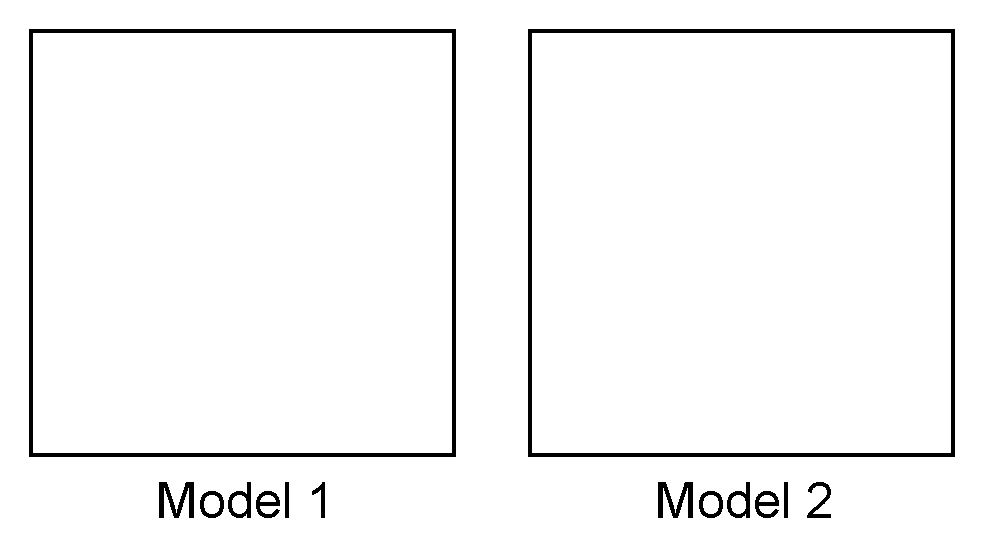
\includegraphics[width=0.6\textwidth]{\figpath/Model1and2_blank.pdf}}}
		\instructordisplay{\centerline{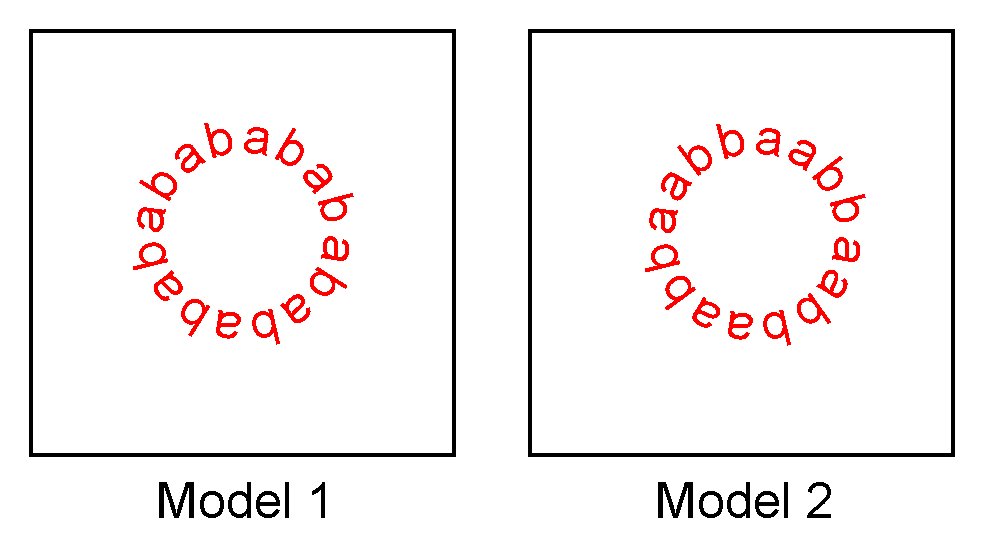
\includegraphics[width=0.4\textwidth]{\figpath/Model1and2_solution.pdf}}}
		
		Note: many students may draw one linear chain with an unreacted `A' group on one end and an unreacted `B' group on the other. This answer will still give them the correct $N_n$, but is not strictly the product that would result if the system reacted until no more reactions can take place.  Ring formation may be worth a brief discussion since rings can be a side product in experimental step-growth polymerizations.
	\end{solution}
		
		\question Calculate the number-average degree of polymerization for both of the ``final'' states you drew in response to the previous question:
		
		\begin{solution}[1in]
			In both models, there is only one molecule in the final state.
			
			Thus, for both models, $N_n = 8/1 = 8$.
		\end{solution}
\end{ctqs}

\begin{model}[A Stoichiometrically-Imbalanced Reaction Mixture]

Practically speaking, it is often very difficult to ensure that a reaction mixture is perfectly stoichiometrically-balanced, and there is often a small excess of one type of monomer or the other.

In this model, consider a reaction mixture that starts with 3 AA-type monomers and 5 BB-type monomers:

\vspace{0.1in}
\centerline{\includegraphics[width=0.4\textwidth]{\figpath/AABBpolym-nonstoich.pdf}}

\end{model}

\begin{ctqs}

		\question Fill in the blank spaces in the figure below with reasonable predictions for what the reaction mixture might look like in each successive step.
		
			\begin{solution}[1in]
				\studentdisplay{\centerline{\includegraphics[width=0.9\textwidth]{\figpath/AABBpolym-nonstoichsteps_blank.pdf}}}
					\instructordisplay{\centerline{\includegraphics[width=0.9\textwidth]{\figpath/AABBpolym-nonstoichsteps_solution.pdf}}}
			\end{solution}
		
		\question Which type of reactive group is the ``limiting reagent'' in this reaction?  Briefly explain your reasoning.
		
			\begin{solution}[1in]
				Each step of the reaction requires an equal number of `A' and `B' reactive groups. Since there are fewer `A' groups in the initial reaction mixture, the `A' reactive groups are the limiting reagent.
			\end{solution}
		
		\question \label{ctq:nonstoichpredict} Predict what the reaction mixture in Model 3 might look like if you let it react until no more reactions could take place:
		
\begin{solution}
\studentdisplay{\centerline{\includegraphics[width=0.3\textwidth]{\figpath/Model3_blank.pdf}}}
\instructordisplay{\centerline{\includegraphics[width=0.3\textwidth]{\figpath/Model3_solution.pdf}}}
\end{solution}
		
		\question Calculate the number-average degree of polymerization for the ``final'' state you drew in response to the previous question:
		
		\begin{solution}[1in]
			There are two molecules in the final reaction mixture, so the number-average degree of polymerization is $N_n = 8/2 = 4$.
		\end{solution}
		
		\question Is the final degree of polymerization for this stoichiometrically-unbalanced reaction smaller than, equal to, or larger than the final degree of polymerization you calculated for the stoichiometrically-balanced reactions in Models 1 and 2?
		
		\begin{solution}[1in]
			$N_n$ for the stoichiometrically-imbalanced reaction is \emph{smaller} than $N_n$ for the stoichiometrically-balanced reactions.
		\end{solution}
		
		\question Which type of reactive group is on the ends of all of the chains you drew in question \ref{ctq:nonstoichpredict}?
		
		\begin{solution}[0.5in]
			All of the chains have `B' groups on the ends.
		\end{solution}
		
		\question Briefly critique or defend the following statement:
		
			\emph{``When drawing the structure of a polymer produced by a step-growth polymerization, we should always make sure that we draw end groups consistent with whichever reactive species was present in excess.''}
		
		\begin{solution}[1.5in]
			DEFEND: in a step growth polymerization, all of the molecules have either `A' groups or `B' groups on either end.  If there is an excess of `B' groups, the reaction will (ideally) go until all of the `A' groups have been used up, leaving only `B' groups on the ends of all of the polymer chains.
		\end{solution}
			
\end{ctqs}
	
\begin{infobox}

In stoichiometrically-imbalanced step-growth polymerizations with an excess of B groups, we define a parameter $r$ that reflects the ratio of A groups to B groups.	
	If the initial number of A groups is $v_A^0$ and the initial number of B groups is $v_b^0$, then
	\begin{equation*}
		r = \frac{v_A^0}{v_B^0}
	\end{equation*}
	
	
	For a reaction mixture with stoichiometric imbalance $r$ at extent of reaction $p$, the number-average degree of polymerization is given by
	\begin{equation*}
		N_n = \frac{1+r}{1+r-2pr}
	\end{equation*}
	
\end{infobox}
	
\begin{ctqs}
		%\question When $r=1$, how can you simplify this expression for $N_n$?		
		%\question When $p=1$, how can you simplify this expression for $N_n$?
		\question Using this expression, fill in the following table with the expected number-average degree of polymerization for different combinations of $r$ and $p$ values:
		
			\begin{table}[!h]
				\centering
				\renewcommand{\arraystretch}{3}
				\begin{tabular}{|c|c|c|c|}
					\hline
					 &  ~$p=0.9$~ & ~$p=0.99$~ & ~$p=0.999$~ \\\hline
					$r=0.9$ & \answer{7} & \answer{16} & \answer{18.7} \\\hline
					$r=0.99$ & \answer{10} & \answer{67} & \answer{166} \\\hline
					$r=0.999$ & \answer{10} & \answer{95} & \answer{667} \\\hline
				\end{tabular}
			\end{table}
		
		\question On the basis of your answers to the previous question, briefly critique or defend the following statement:
		
			\emph{``Achieving high molecular weights in step-growth polymerizations requires both very precise measurement of the reagents, and reaction conditions which strongly favor the bond-forming reaction.''}
			
			\begin{solution}[1.5in]
				DEFEND: As we can see from the table in the previous question, achieving a large degree of polymerization requires \emph{both} $r$ and $p$ to be close to $1$.
				Since $r$ reflects the reagent ratio, this means that we must measure the reagents very precisely to get as close to perfect stoichiometric balance as possible.
				Since $p$ reflects the extent of reaction, or the fraction of reactive groups that have reacted, getting $p$ close to 1 requires being able to push the $A+B\to ab$ reaction as far toward the products as possible.
			\end{solution}
			
\end{ctqs}

\begin{exercises}

		\exercise In the stoichiometrically-balanced reactions in models 1 and 2, the number of molecules was always equal to the number of unreacted `A' groups.  Is the same thing true for the stoichiometrically-imbalanced reaction in Model 3? Why or why not? % if not, how could you modify?
		
			\begin{solution}
				No, the same is not true for the stoichiometrically-imbalanced reaction in Model 3.  
				
				The key here is to realize that each step of the reaction does two things:
				\begin{enumerate}
					\item it uses up one `A' reactive group (and one `B' reactive group, but we're only counting `A' groups here)
					\item it decreases the total number of molecules in the reaction by one (it takes two molecules and links them together to form one)
				\end{enumerate}
				In Models 1 and 2, the stoichiometric balance means that the initial number of `A' groups is equal to the intial number of molecules.
				In each step, both of the number of unreacted `A' groups and the number of molecules decrease by one, so the number of `A' groups is always exactly equal to the number of molecules.
				
				In Model 3, however, the stoichiometric imbalance means that the initial number of `A' groups is smaller than the initial number of molecules.
				While the number of unreacted `A' groups and the number of molecules still both decrease by one in each step, they are not equal to each other since the initial values were not equal.
				
			\end{solution}
	
		\exercise In this activity, we only calculated the number-average \emph{degree of polymerization} of the polymers produced in step-growth polymerizations. However, usually, we want to be able to calculate the \emph{molecular weight} of the polymers as well.
		
			\begin{enumerate}
			
				\item In Model 1, we considered a reaction of AB-type monomers.  If each monomer had mass $m_{AB}$, how would you calculate the number-average molecular weight, $M_n$, of the polymer produced when the extent of reaction is equal to $p$?
				
					\begin{solution}
						Recall that, in general,
						\begin{equation*}
							M_n = M_0 N_n
						\end{equation*}
						where $M_0$ is the molecular weight of a single monomer and $N_n$ is the number of monomers.
						
						Here, the molecular weight of the monomer is $m_{AB}$, so
						\begin{equation*}
							M_n = m_{AB} N_n = \frac{m_{AB}}{1-p}
						\end{equation*}
					\end{solution}
				
				\item In Model 2, we considered a stoichiometrically-balanced reaction of AA- and BB-type monomers. If the AA-type monomers each had mass $m_{AA}$ and the BB-type monomers each had mass $m_{BB}$, how would you calculate the number-average molecular weight of the polymer produced when the extent of reaction is equal to $p$?
				
					\emph{Note: this question is a little tricky - remember that $N_n$ counts \emph{monomers}, but in this reaction, not all of the monomers have the same molecular weight.  How might you be able to correct for this?}
					
					\begin{solution}
						To address this problem, we'll assume that on average, half of the monomers in each polymer chain will be AA-type monomers and half will be BB-type monomers (this is generally a reasonable assumption, except at very low degrees of polymerization).
						
						In this case, the average number of AA-type monomers in a given polymer chain is $N_n/2$, so their contribution to the molecular weight is $m_{AA}\frac{N_n}{2}$.  Similarly, the average number of BB-type monomers in a given polymer chain is also $N_n/2$, so their contribution to the molecular weight is $m_{BB}\frac{N_n}{2}$.
						
						Put together, the total molecular weight is
						\begin{align*}
							M_n &= m_{AA}\frac{N_n}{2} + m_{BB}\frac{N_n}{2}\\
								&= \frac{m_{AA} + m_{BB}}{2} N_n\\
								&= \frac{m_{AA} + m_{BB}}{2} \frac{1}{1-p}
						\end{align*}
						
						Note that the second line of this expression looks a lot like $M_n = M_0 N_n$, but with $M_0 = \frac{m_{AA} + m_{BB}}{2}$.  Thus, one way to interpret this result is to say that the number-average molecular weight is the number-average degree of polymerization times the \emph{average} molecular weight of the monomers.
					\end{solution}
				
			\end{enumerate}
		
		\exercise In Model 3, we considered a stoichiometrically-imbalanced reaction of AA- and BB-type monomers.  However, another important limit occurs when we have equal numbers of AA- and BB-type monomers, but add in an extra monofunctional reagent ``Bx'' that can only react on one side.
		
			In this exercise, suppose that we have $v_A^0$ `A' groups from AA-type monomers, $v_B^0$ `B' groups from BB-type monomers, and $v_{B'}^0$ `B' groups from Bx-type molecules.
		
			\begin{enumerate}
				\item Consider the following statements from two students:
					
					\begin{itemize}
				
					\item \textbf{Student 1:} \emph{``The total number of `B' groups is just $v_B^0 + v_{B'}^0$, so we can account for the presence of monofunctional Bx molecules by replacing $r=\frac{v_A^0}{v_B^0}$ with $r'=\frac{v_A^0}{v_B^0 + v_{B'}^0}$.''}
					
					\item \textbf{Student 2:} \emph{``One Bx molecule has the same effect on the degree of polymerization as one BB-type molecule.  Since Bx-type molecules have the same effect with half as many `B' groups, that means that a `B' group from a Bx molecule is twice as effective at stopping chain growth as a `B' group from a BB molecule, so we should replace $r$ with $r'=\frac{v_A^0}{v_B^0 + 2v_{B'}^0}$.''}
					\end{itemize}
					
					Which student do you agree with, and why?
				
					\begin{solution}
						Student 2 is correct.  Because extra BB-type and Bx-type molecules both effectively terminate a chain end and stop it from growing, one Bx-type molecule has the same effect on the degree of polymerization as one BB-type molecule.  As a result, the individual `B' groups in the BB-type molecule are essentially half as effective as the single `B' group in the Bx-type molecule, or, conversely, the `B' group in the Bx molecule is twice as effective as each `B' group from the BB-type molecules.
						
						One way to see this is to consider the simple reaction of one AA molecule with two Bx molecules.  In this case, when the reaction has gone all the way to completion, we should get a `xbaabx' oligomer.  This is essentially the same result that we would get from a reaction of one AA molecule with two BB molecules, which would result in a 'BbaabB' oligomer.  In both cases we end up with the same final degree of polymerization, even though we had twice as many `B' groups in the second case.
						
					\end{solution}
				
				\item Monofunctional reagents are a common impurity in supplies of difunctional monomers. Briefly explain why this means it is necessary to rigorously purify the starting materials used in step-growth polymerizations.
				
					\begin{solution}
						As seen above, monofunctional molecules are very effective at capping polymer chains and preventing the reaction from going further.  In a stoichiometrically-balanced reaction, if even just 5\% of the `B' groups come from monofunctional reagents, the average degree of polymerization will be capped at about 40 monomers, which is too short to be of much use in practical applications.
					\end{solution}
			\end{enumerate}
\end{exercises}
	
\end{activity}

	\chapter{Free-Radical Polymerization}

	\chapter{Controlled Polymerizations}

	\chapter{Copolymers}

\part{Polymer Physics}

	\chapter{Conformations of Polymer Chains}

	\chapter{Mechanical Properties of Polymers}

	\chapter{Phase Behavior of Polymers \& Their Solutions}

	\chapter{Thermal Properties of Polymers}


%\appendix

%\chapter{An Appendix Chapter}

%\lipsum[1-15]

\backmatter

\end{document}